\documentclass{pre-tfg}
\usepackage{url}
\usepackage{graphicx}

% \showhelp  % comenta o borra para eliminar ayudas

\title{Sense: Plataforma de alto rendimiento para captura y procesado de eventos IoT}
\author{David Martín García}
\advisorFirst{David Villa Alises}
\advisorDepartment{Tecnologias y sistemas de información}
\advisorSecond{Maria Jose Santofimia Romero}
\intensification{COMPUTACIÓN}
\docdate{2015}{Noviembre}

\def\FIXME #1 {\textcolor{red}{\textbf{FIXME:}} #1}

\begin{document}

\maketitle
\tableofcontents

\newpage

\section{INTRODUCCIÓN}

La sociedad avanza hacia una nueva era en la que Internet tiene un papel aún más
importante. En los últimos años estamos experimentando un crecimiento exponencial en la
cantidad de datos volcados en Internet así como en el número de dispositivos que generan o
consumen tal información. En ámbitos como los sistemas multiagente o la minería de datos
se manejan conceptos como la ubicuidad o \emph{Big Data} que se considerar premisas de
futuro, y que están íntimamente relacionados con la manipulación y extracción de
conocimiento a partir de cantidades masivas de datos.

Todo está interconectado y tecnologías como la domótica, el ocio o la salud están muy
influidas por esta tendencia. Hoy en día, dispositivos como smart watches, smart bands,
smart phones o smart TVs se conectan a Internet para consumir y publicar datos, desde
tendencias de uso hasta datos personales de nuestra salud o ejercicio físico. Por otro
lado, empresas de multitud de ámbitos consumen y publican datos para uso interno. Empresas
de logística, automatización de entornos domésticos e industriales, generación y
distribución de energía eléctrica, automóvil, telecomunicaciones e información. Todos
estos campos se ven cada vez mas influenciados por esta tecnología.

Solo hay que imaginar una cadena logística, donde una gran cantidad de sensores y
actuadores funcionan de forma conjunta para proveer de información, tanto al usuario como
al propio funcionamiento de la empresa.

Cada día se ve mas presente mercados influenciados por tecnologías M2M (Machine to
Machine) donde la interacción es únicamente entre dispositivos (sin intervención
humana). Empresas como Cisco prevén 50 billones de dispositivos conectados a
Internet. Esta ingente cantidad de datos conlleva grandes problemas de almacenamiento, así
como un requisito esencial: la optimalidad. El número de conexiones crece
exponencialmente, tanto que son necesarios nuevos protocolos como IPv6, que proporciona 340
sextillones de direcciones. Esto hace intuir que no es una simple moda o tendencia que se
disipara en unos años, es una necesidad, y empresas como
IBM\footnote{http://www.ibmbigdatahub.com/technology/internet-of-things}, Microsoft o
Intel\footnote{https://software.intel.com/es-es/iot/microsoft-azure} apuestan por
ello. Otras empresas como Ericson, Siemens Bosch tienen las tecnologias IoT como punta de
lanza en las presentaciones de sus tecnologías mas novedosas.

Todo esto hace prever que no es solo un cambio de tendencia temporal, es uno de los
mayores campos de investigación y negocio en los próximos años. Es considerado por muchos
como una de las innovaciones disruptivas más importantes en la actualidad.

Por otro lado, el número de hubs de datos ha crecido de manera exponencial, así como su
valor en el mercado, dado que existe una gran demanda de este tipo de servicios.

Al hacer referencia al término \emph{hub de datos}, entendemos estos como la infraestructura necesaria para el correcto almacenamiento de datos heterogéneos, donde posteriormente pueden ser visualizados, distribuidos y compartidos.

Y es en ese punto donde encaja este proyecto. Se trata de crear un \emph{hub de datos},
donde poder publicar y consumir toda esta información. La principal meta de este proyecto
es la optimización de este proceso del proceso de publicación y consumo, así como el
análisis de los datos, dos de los principales hitos en la mayoría de Hubs actuales. Este
hub será de carácter gratuito y \emph{open source}. Mezclará tecnologías y lenguajes de
forma heterogénea, donde cada uno es el mejor en su campo, todos ellos en conjunto
formaran un conjunto de micro-servicios, interrelacionados entre si.

Las premisas del proyecto están principalmente marcadas por la tasa de ingestión de datos
así como la posibilidad de realizar operaciones a un bajo costo computacional, operaciones
como el análisis de los datos.


\section{TECNOLOGÍA ESPECÍFICA / INTENSIFICACIÓN / ITINERARIO CURSADO POR EL ALUMNO}

\begin{table}[hp]
  \centering
  \caption{Tecnología Específica cursada por el alumno}
  \label{tab:tec-especifica}

  \zebrarows{1}
  \begin{tabular}{p{0.01\linewidth}p{0.4\linewidth}}
    &\textbf{Marcar la tecnología cursada} \\
    \hline
    & Tecnologías de la Información \\
    \textbf{*} &\textbf{Computación} \\
    &Ingeniería del Software \\
    &Ingeniería de Computadores \\
    \hline
  \end{tabular}
\end{table}


\begin{table}[hp]
  \centering
  \caption{Justificación de las competencias específicas abordadas en el TFG}
  \label{tab:competencias}

  \zebrarows{1}
  \begin{tabular}{p{0.5\linewidth}p{0.5\linewidth}}
    \textbf{Competencia} & \textbf{Justificación} \\
    \hline
    Capacidad para adquirir, obtener, formalizar y representar el conocimiento humano en
    una forma computable para la resolución de problemas mediante un sistema informático
    en cualquier ámbito de aplicación, particularmente los relacionados con aspectos de
    computación, percepción y actuación en ambientes entornos inteligentes.
    & Al tratar con valores de cualquier forma, como por ejemplo
    sensores, debemos comprender las diferentes magnitudes así como una
    posible forma normal para poder comparar entre los distintos valores.\\
    %
    Capacidad para desarrollar y evaluar sistemas interactivos y de
    presentación de información compleja y su aplicación a la resolución
    de problemas de diseño de interacción persona computadora.
    & Desarrollo de entorno gráfico donde poder monitorizar los datos
    así como las distintas opciones y incidencias que se detecten,
    además de la gestión de perfiles de usuario así como de los
    distintos metadatos asociados a la entrada de datos.\\
    %
    Capacidad para conocer y desarrollar técnicas de aprendizaje computacional y diseñar e
    implementar aplicaciones y sistemas que las utilicen, incluyendo las dedicadas a
    extracción automática de información y conocimiento a partir de grandes volúmenes de
    datos.
    & Análisis de los datos obtenidos así como  detección de valores anormales y obtención
    de posibles respuestas ante tal estimulo.\\
    %
    Capacidad para evaluar la complejidad computacional de un problema, conocer
    estrategias algorítmicas que puedan conducir a su resolución y recomendar, desarrollar
    e implementar aquella que garantice el mejor rendimiento de acuerdo con los requisitos
    establecidos.
    & Diseño y implementación de algoritmo de agrupamiento de datos. Este algoritmo
    agregara los diferentes datos con el fin de mantener controlado el tamaño máximo de la
    base de datos.\\
    \hline
  \end{tabular}
\end{table}
 \clearpage

\section{OBJETIVOS}

Desarrollo de un hub para el almacenamiento de datos con carácter temporal orientado al
concepto IoT (Internet of Things).

Se debe plantear un arquitectura de micro-servicios de alto rendimiento. Se plantea una
parte central que permita el almacenamiento, análisis y tratamiento de los datos, así como
servicios en torno a ésta para las notificaciones a los distintos dispositivos que
requieran de estos datos.

Deben existir servicios de notificación, análisis, autenticación además de la gestión y
almacenamiento de los datos así como su consulta.

También se requiere de una interfaz gráfica de gestión que se desarrolla mediante una
aplicación web, asegurando así su total compatibilidad con la gran mayoría de dispositivos
existente.

Debe tener compatibilidad con los estándares de comunicación como REST, MQTT o ZeroC Ice.

Se debe disponer de una API para la comunicación con los distintos dispositivos externos,
así como un protocolo de comunicación para la parte interna entre servicios.

Se tendrá el cuenta el rendimiento como principal punto de selección en la infraestructura
así como en cada parte del proyecto, debido a esto se prevé un desarrollo metalenguaje
como punto principal para la búsqueda de este objetivo.

También se desarrollara el aprovisionamiento de servidores así como la disposición de un
entorno de desarrollo de fácil instalación para cualquier desarrollador.

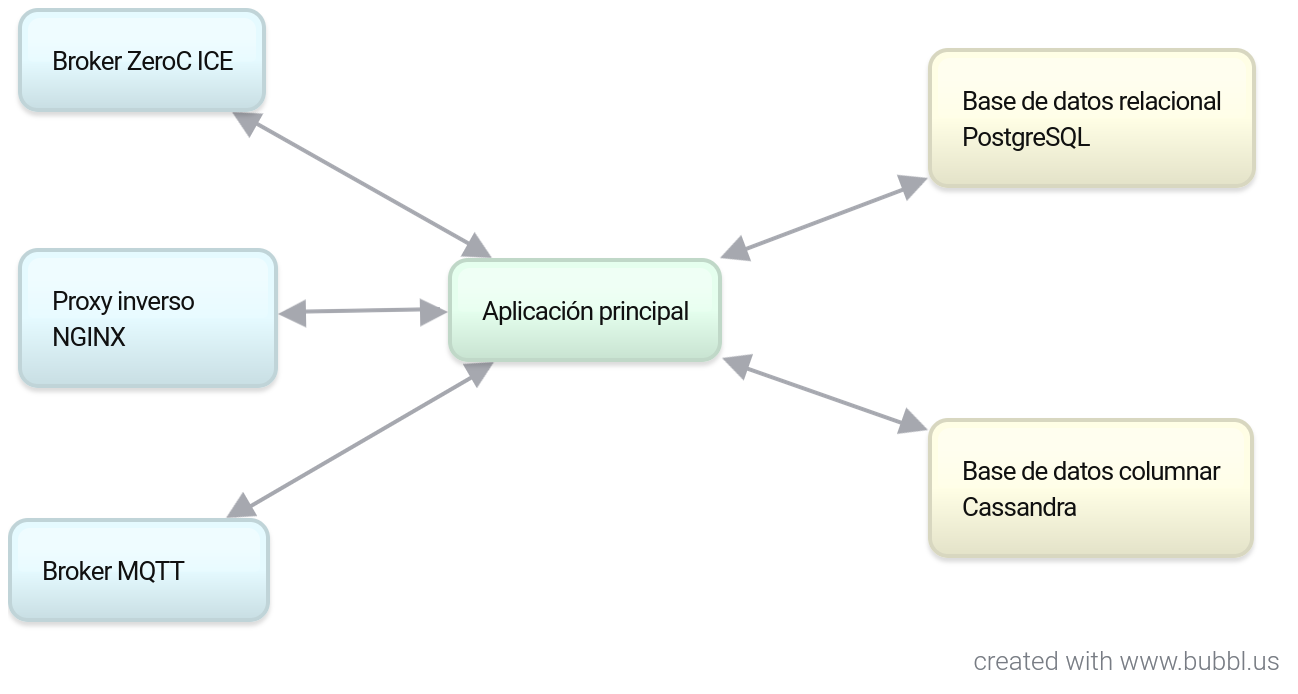
\includegraphics{grafico-arquitectura.png}

\section{MÉTODO Y FASES DE TRABAJO}

Para llevar a cabo este proyecto se realizado un análisis previo de las diversas
metodologías existentes.

La elección de una metodología ágil es fiel reflejo de la naturaleza de este proyecto,
donde a fecha inicial no se define totalmente los requisitos con total exactitud y donde
la planificación a corto plazo cobra un mayor sentido.

Tras obtener las ventajas e inconvenientes de cada una se ha optado por scrumban, una
mezcla entre Kanban y Scrum, donde se pactaran diferentes hitos dentro del plazo máximo
para desarrollar el proyecto, cumpliendo con diferentes \emph{sprints}, pero a su vez
haciendo uso de Kanban como planificación de las diferentes tareas.

Con esto tenemos las ventajas de ambos, por un lado controlamos el progreso en casa
sprint, y nos permite a su vez gestionar las tareas mediante un tablón Kanban, obteniendo
la mínima latencia desde el desarrollo hasta la integración con su versión de
producción. Además nos permite seguir las diferentes fases del software, desde el diseño,
hasta su puesta al publico, pasando por las fases de codificación, test, aceptación y
calidad.

Esta metodología nos permite adaptarnos mejor a los cambios en los requisitos o en el ritmo
de trabajo, ya que por la propia naturaleza del proyecto, debe compaginarse con el resto de
actividades académicas.

\FIXME{TODO: DEFINIR HITOS A GRANDES RASGOS, es por hacerme una idea del tamaño Corregir
  si o si.....}

\begin{itemize}
\item Hito 1 - Analisis
  \begin{itemize}
  \item
  \item
  \item Realización de la documentación inicial y puesta a punto de los
    diferentes servicios involucrados en el desarrollo
  \end{itemize}

\item Hito 2
  \begin{itemize}
  \item Análisis de rendimiento de las diferentes propuestas, así como la
    obtención de una primera estadística de rendimiento esperado del proyecto en cada
    una de sus partes.
  \item Codificación del núcleo de micro-servicios
  \item Obtención de la primera versión funcional
  \end{itemize}

\item Hito 3
  \begin{itemize}
  \item Desarrollo de la interfaz web
  \item Desarrollo del backend de análisis de datos
  \end{itemize}
\end{itemize}

\clearpage
\section{MEDIOS QUE SE PRETENDEN UTILIZAR}

\subsection{Medios Hardware}

Para la realización de este proyecto se van a utilizar los siguientes medios hardware, se
estructuraran en los diversos entornos disponibles:

\textbf{Desarrollo}:
Entorno de desarrollo, donde se realizan las tareas de codificación.

\begin{table}[hp]
  \caption{Características del entorno de desarrollo}
  \centering
  \zebrarows{1}

  \begin{tabular}{p{0.2\linewidth}p{0.4\linewidth}}
    & MacBook Pro 2014 Mid.\\
    CPU& Intel i5 4308U @ 2.8Ghz.\\
    RAM& 8GB DDR3L 1600Mhz.\\
    Almacenamiento& SSD M2 128GB.\\
    SO& Debian 8.2.\\
  \end{tabular}
\end{table}

\textbf{Staging}

Servidor local donde se realizaran las distintas pruebas a la plataforma para comprobar su
funcionamiento, además realiza las funciones de servidor publico donde se alojara la
plataforma.

\begin{table}[hp]
  \caption{Características del entorno de staging}
  \centering
  \zebrarows{1}

  \begin{tabular}{p{0.2\linewidth}p{0.4\linewidth}}
    CPU& Intel i5 4690K @ 5Ghz.\\
    RAM& 16GB DDR3 1833Mhz.\\
    Almacenamiento& SSD 120GB + RAID0 2TB (2 discos de 1TB).\\
    SO& Debian 8.2.\\
  \end{tabular}
\end{table}

\textbf{Producción}

Servidor dedicado donde se encuentra el entorno publico, este entorno es el que
disfrutaran los usuarios.

\begin{table}[hp]
  \caption{Características del entorno de producción}
  \centering
  \zebrarows{1}

  \begin{tabular}{p{0.2\linewidth}p{0.4\linewidth}}
    CPU& Intel Xeon E5 2620V2.\\
    RAM& 32GB DDR3 ECC.\\
    Almacenamiento& 3x SSD 256GB (RAID0) + 100GB (Backups).\\
    SO& Debian 8.3.\\
  \end{tabular}
\end{table}

\clearpage
\subsection{Medios Software}

\begin{itemize}
\item Control de versiones: Git.
\item Comunicación entre las distintas partes: Slack.
\item Técnicas de diseño e implementación software: TDD.
\item Servicios de integración continua: TravisCI ó CircleCI.
\item Lenguaje: Elixir, C, Python, Ruby, JavaScript, HTML5.
\item Entorno de desarrollo: Emacs.
\end{itemize}

Además, se prevé utilizar las siguientes tecnologías en la capa de persistencia:

\begin{itemize}
\item Base de datos: NoSQL con escalabilidad en horizontal así como un
  tiempo medio de respuesta bajo en las inserciones. Se prevé utilizar Cassandra.
\item Persistencia temporal: Redis.
\end{itemize}


\section{REFERENCIAS}

\FIXME{Las referencias son MUY
  importantes en el anteproyecto. Debes \textbf{citar} en la introducción al menos 6 o 7
  artículos o revistas de investigación que traten el tema de IoT, manipulación de datos
  masiva y otros aspectos esenciales del proyecto.}

\begin{itemize}
  \item Big Data Platforms for the Internet of Things~\cite{Ciobanu2014}.
  \item Big Data and the Internet of Things~\cite{Shah2016}.
  \item New Horizons for a Data-Driven Economy: A Roadmap for Usage and Exploitation of Big Data in Europe~\cite{Strohbach2016}.
  \item Components and Services for IoT Platforms~\cite{CaSfIotPlatforms17}.
  \item Enable things to talk, Springer~\cite{EIoT2Talk13}.
\end{itemize}

\bibliographystyle{alpha}
\bibliography{main}

\end{document}

% Local Variables:
% coding: utf-8
% mode: flyspell
% ispell-local-dictionary: "castellano8"
% mode: latex
% End:


%http://www.erol.si/2015/01/the-complete-list-of-all-timeseries-databases-for-your-iot-project/
%http://www.infoworld.com/article/2825890/application-development/why-redis-beats-memcached-for-caching.html
%http://phoenix.thefirehoseproject.com/0.html
%https://github.com/trenpixster/addict
%https://github.com/opendrops/passport
%http://safecast.org/tilemap/
%https://es.wikipedia.org/wiki/IPv6
%http://cassandra.apache.org/
%http://stackoverflow.com/questions/410616/increasing-the-maximum-number-of-tcp-ip-connections-in-linux

%(IOT CASSANDRA - https://www.instaclustr.com/customers/iot/,
%https://spark-summit.org/2014/wp-content/uploads/2014/07/Using-Spark-Streaming-for-High-Velocity-Analytics-on-Cassandra-Albert-Tobey-Tupshin-Harper.pdf,
%http://www.datastax.com/internet-of-things,
%http://www.planetcassandra.org/blog/functional_use_cases/internet-of-things-sensor-data/,
%http://highscalability.com/blog/2010/7/11/so-why-is-twitter-really-not-using-cassandra-to-store-tweets.html,
%)

%  LocalWords:  Intel ademas domótica smart multiagente metadatos Kanban
